\documentclass[tikz,border=8pt]{standalone}
% Shared look for every TikZ diagram. Load with \input{../../tools/tikz-style.tex}
\usepackage[T1]{fontenc}
\usepackage{lmodern}
\renewcommand{\sfdefault}{lmr}  % diagrams use the same serif as the text
\usetikzlibrary{arrows.meta, positioning, shapes.geometric, calc, fit, backgrounds}
\definecolor{cblue}{HTML}{4C78A8}
\definecolor{corange}{HTML}{F58518}
\definecolor{cgreen}{HTML}{54A24B}
\definecolor{cred}{HTML}{E45756}
\definecolor{cpurple}{HTML}{B279A2}
\definecolor{cgrey}{HTML}{6B6B6B}
\tikzset{
  every picture/.style={font=\sffamily, line width=1.2pt},
  box/.style={draw=#1, fill=#1!12, rounded corners=4pt, align=center, inner sep=7pt, minimum height=1.1cm},
  box/.default=cgrey,
  arrow/.style={-{Stealth[length=3mm]}, draw=cgrey, line width=1.4pt},
  title/.style={font=\sffamily\bfseries\Large},
  note/.style={font=\sffamily\small, text=cgrey, align=center},
}
\AtBeginDocument{\hyphenpenalty=10000 \exhyphenpenalty=10000}

\begin{document}
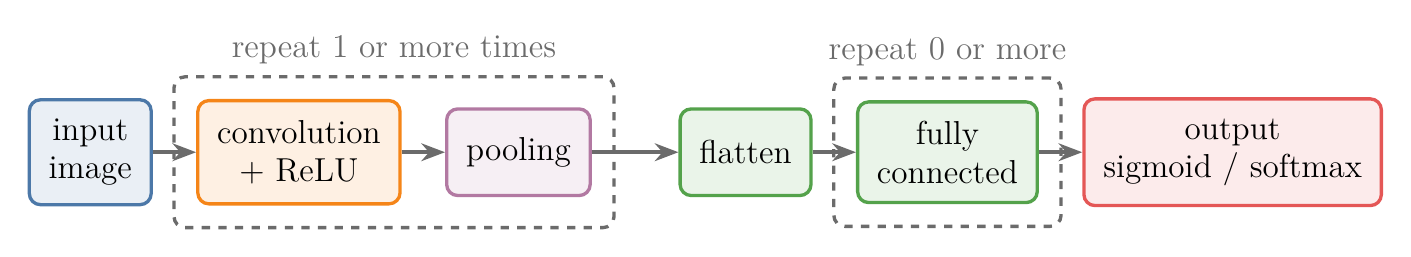
\begin{tikzpicture}[node distance=0.55cm, every node/.append style={font=\sffamily\large}]
  \node[box=cblue] (in) {input\\image};
  \node[box=corange, right=of in] (c) {convolution\\+ ReLU};
  \node[box=cpurple, right=of c] (p) {pooling};
  \node[box=cgreen, right=1.1cm of p] (f) {flatten};
  \node[box=cgreen, right=of f] (fc) {fully\\connected};
  \node[box=cred, right=of fc] (o) {output\\sigmoid / softmax};
  \draw[arrow] (in) -- (c); \draw[arrow] (c) -- (p); \draw[arrow] (p) -- (f); \draw[arrow] (f) -- (fc); \draw[arrow] (fc) -- (o);
  \node[draw=cgrey, dashed, rounded corners, fit=(c)(p), inner sep=8pt, label={[text=cgrey]above:repeat 1 or more times}] {};
  \node[draw=cgrey, dashed, rounded corners, fit=(fc), inner sep=8pt, label={[text=cgrey]above:repeat 0 or more}] {};
\end{tikzpicture}
\end{document}
